\documentclass[border=1pt]{standalone}
\usepackage{tikz}
\usepackage{tikz-3dplot}
\usetikzlibrary{calc}

\begin{document}
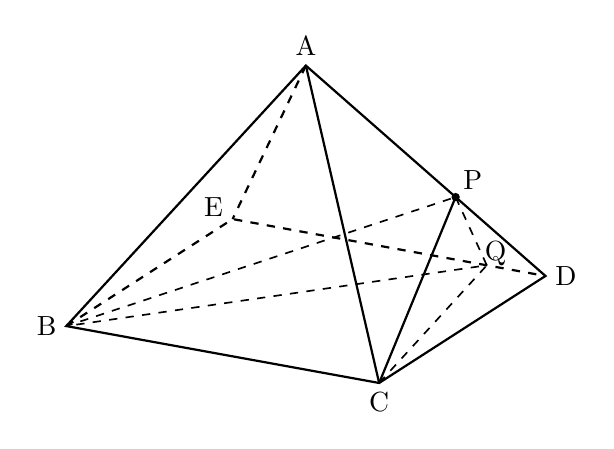
\begin{tikzpicture}
    \tdplotsetmaincoords{70}{118}
    \begin{scope}[tdplot_main_coords]
        
        % パラメータの定義
        \pgfmathsetmacro{\X}{4.5}
        \pgfmathsetmacro{\Y}{\X}
        \pgfmathsetmacro{\Z}{\X/2*sqrt(2)}
        \pgfmathsetmacro{\da}{0.12*\X}
        \pgfmathsetmacro{\db}{0.25*\X}
        \pgfmathsetmacro{\dc}{0.05*\X}

        % 頂点の座標の定義
        \coordinate (E) at (0,0,0); 
        \coordinate (B) at (\X,0,0); 
        \coordinate (C) at (\X,\Y,0);
        \coordinate (D) at (0,\Y,0);
        \coordinate (A) at (\X/2,\Y/2,\Z);
        \coordinate (P) at ($(A)!0.625!(D)$);
        \coordinate (Q) at ($(E)!0.8125!(D)$);

        % 頂点のラベル
        \node[left, yshift=4*\db] at (E) {E};
        \node[left] at (B) {B};
        \node[below] at (C) {C};
        \node[right] at (D) {D};
        \node[above] at (A) {A};
        \node[above right, outer sep=-.5pt] at (P) {P};
        \node[xshift=2.8*\db, yshift=3.8*\db] at (Q) {Q};

        % 線・点の描画
        \draw [thick] (A) -- (B) -- (C) -- (D) -- cycle;
        \draw [thick] (A) -- (C);
        \draw [thick] (C) -- (P);
        \draw [thick,dashed] (B) -- (E) -- (D);
        \draw [thick,dashed] (A) -- (E);
        \draw [semithick,dashed] (P) -- (Q) -- (B) -- cycle;
        \draw [semithick,dashed] (C) -- (Q);
        \fill (P) circle (1.5pt);
    
    \end{scope}
 
\end{tikzpicture}
\end{document}

